% Choose one to switch between slides and handout
%\documentclass[]{beamer}
\documentclass[handout]{beamer}

% Video Meta Data
\title{Bitcoin, Blockchain and Cryptoassets}
\subtitle{Intro: Welcome to the Course}
\author{Prof. Dr. Fabian Schär}
\institute{University of Basel}

% Config File
% Packages
\usepackage[utf8]{inputenc}
\usepackage{hyperref}
\usepackage{gitinfo2}
\usepackage{tikz}
\usepackage{amsmath}
\usepackage{mathtools}
\usepackage{bibentry}
\usepackage{xcolor}
\usepackage{colortbl} % Add colour to LaTeX tables
\usepackage{caption}
\usepackage[export]{adjustbox}
\usepackage{pgfplots} \pgfplotsset{compat = 1.17}
\usepackage{makecell}
\usepackage{fancybox}
\usepackage{ragged2e}
\usepackage{fontawesome}
\usepackage{seqsplit}
\usepackage{tabularx}

% Color Options
\definecolor{highlight}{rgb}{0.65,0.84,0.82}
\definecolor{focus}{rgb}{0.72, 0, 0}
\definecolor{lightred}{rgb}{0.8,0.5,0.5}
\definecolor{midgray}{RGB}{190,195,200}

% Beamer Template Options
\beamertemplatenavigationsymbolsempty
\setbeamertemplate{footline}[frame number]
\setbeamercolor{structure}{fg=black}
\setbeamercolor{footline}{fg=black}
\setbeamercolor{title}{fg=black}
\setbeamercolor{frametitle}{fg=black}
\setbeamercolor{item}{fg=black}
\setbeamercolor{}{fg=black}
\setbeamercolor{bibliography item}{fg=black}
\setbeamercolor*{bibliography entry title}{fg=black}
\setbeamercolor{alerted text}{fg=focus}
\setbeamertemplate{items}[square]
\setbeamertemplate{enumerate items}[default]
\captionsetup[figure]{labelfont={color=black},font={color=black}}
\captionsetup[table]{labelfont={color=black},font={color=black}}

\setbeamertemplate{bibliography item}{\insertbiblabel}

% Link Icon Command
\newcommand{\link}{%
    \tikz[x=1.2ex, y=1.2ex, baseline=-0.05ex]{%
        \begin{scope}[x=1ex, y=1ex]
            \clip (-0.1,-0.1)
                --++ (-0, 1.2)
                --++ (0.6, 0)
                --++ (0, -0.6)
                --++ (0.6, 0)
                --++ (0, -1);
            \path[draw,
                line width = 0.5,
                rounded corners=0.5]
                (0,0) rectangle (1,1);
        \end{scope}
        \path[draw, line width = 0.5] (0.5, 0.5)
            -- (1, 1);
        \path[draw, line width = 0.5] (0.6, 1)
            -- (1, 1) -- (1, 0.6);
        }
    }

% Read Git Data from Github Actions Workflow
% Defaults to gitinfo2 for local builds
\IfFileExists{gitInfo.txt}
	{\input{gitInfo.txt}}
	{
		\newcommand{\gitRelease}{(Local Release)}
		\newcommand{\gitSHA}{\gitHash}
		\newcommand{\gitDate}{\gitAuthorIsoDate}
	}

% Custom Titlepage
\defbeamertemplate*{title page}{customized}[1][]
{
  \vspace{-0cm}\hfill\includegraphics[width=2.5cm]{../config/logo_cif}
  \includegraphics[width=1.9cm]{../config/seal_wwz}
  \\ \vspace{2em}
  \usebeamerfont{title}\textbf{\inserttitle}\par
  \usebeamerfont{title}\usebeamercolor[fg]{title}\insertsubtitle\par  \vspace{1.5em}
  \small\usebeamerfont{author}\insertauthor\par
  \usebeamerfont{author}\insertinstitute\par \vspace{2em}
  \usebeamercolor[fg]{titlegraphic}\inserttitlegraphic
    \tiny \noindent \texttt{Release Ver.: \gitRelease}\\ 
    \texttt{Version Hash: \gitSHA}\\
    \texttt{Version Date: \gitDate}\\ \vspace{1em}
    
    
    \iffalse
  \link \href{https://github.com/cifunibas/Bitcoin-Blockchain-Cryptoassets/blob/main/slides/intro.pdf}
  {Get most recent version}\\
  \link \href{https://github.com/cifunibas/Bitcoin-Blockchain-Cryptoassets/blob/main/slides/intro.pdf}
  {Watch video lecture}\\ 
  
  \fi
  
  \vspace{1em}
  License: \texttt{Creative Commons Attribution-NonCommercial-ShareAlike 4.0 International}\\\vspace{2em}
  \includegraphics[width = 1.2cm]{../config/license}
}


% tikzlibraries
\usetikzlibrary{decorations.pathreplacing}
\usetikzlibrary{decorations.markings}
\usetikzlibrary{positioning}
\usetikzlibrary{calc}
\captionsetup{font=footnotesize}


%%%%%%%%%%%%%%%%%%%%%%%%%%%%%%%%%%%%%%%%%%%%%%
%%%%%%%%%%%%%%%%%%%%%%%%%%%%%%%%%%%%%%%%%%%%%%
\begin{document}

\thispagestyle{empty}
\begin{frame}[noframenumbering]
	\titlepage
\end{frame}

%%%
\begin{frame}{Course Structure 1}
\footnotesize

\textbf{1. Introductory Part:}
	\begin{itemize}
		\item Introduction to the Class
		\item Foundations of Monetary Theory
		\item Payment Systems
		\item Monetary Control Structures
		\item Bitcoin Primer
	\end{itemize}
	
\vspace{0.5em}

\textbf{2. Transaction Capacity:}
	\begin{itemize}
		\item Peer-to-Peer Networks
		\item The Bitcoin Network
	\end{itemize}
	
\vspace{0.5em}	
	
	\textbf{3. Introduction to Cryptography:}
	\begin{itemize}
		\item Hash Functions
		\item Symmetric Cryptography
		\item Asymmetric Cryptography
		\item Elliptic Curve Cryptography
	\end{itemize}

	
\end{frame}

\begin{frame}{Course Structure 2}
\footnotesize

\textbf{4. Transaction Legitimacy:}
	\begin{itemize}
		\item Transactions
		\item Bitcoin Script and Standard Transactions
		\item Sig Hash Types
	\end{itemize}	
	
\vspace{0.5em}

\textbf{5. Transaction Consensus:}
	\begin{itemize}
		\item Block Assembly and Chain Structure
		\item Proof-of-Work
		\item Fork Theory
		\item Incentives and Potential Attacks
		\item Alternative Consensus Protocols
	\end{itemize}

\vspace{0.5em}

\textbf{6. Bitcoin as Money:}
	\begin{itemize}
		\item History of Digital Money
		\item Bitcoin Volatility and Pricing Models
		\item CBDC and Stablecoins
	\end{itemize}
	
\end{frame}
%%%

%%%
\begin{frame}{Interdisciplinary Approach}
	\uncover<1->{
		\begin{figure}[h]
  			\center
			\def\firstcircle{(90:1.75cm) circle (2.5cm)}
\def\secondcircle{(210:1.75cm) circle (2.5cm)}
\def\thirdcircle{(330:1.75cm) circle (2.5cm)}
    
\begin{tikzpicture}[scale = 0.67]
	\begin{scope}
    	\clip \secondcircle;
    	\clip \thirdcircle;
    	\fill[highlight] \firstcircle;
    \end{scope}
    \draw \firstcircle node[text=black,above] {\scriptsize{Cryptography}};
    \draw \secondcircle node [text=black,below left] {\scriptsize{Economics}};
    \draw \thirdcircle node [text=black, below right, align=left] {\scriptsize{Computer} \\
    \scriptsize{Science}};
\end{tikzpicture}

		\end{figure}
	}
	\vspace{1em}
Bitcoin and public Blockchains can only be fully understood, when they are studied from various perspectives. This is the reason why this class uses an \color{focus} \textbf{interdisciplinary} \color{black} approach.	
\end{frame}
%%%


%%%
\begin{frame}{Recommended Literature}
	\uncover<1->{
		\begin{columns}[T]
			\begin{column}{0.1\textwidth}
					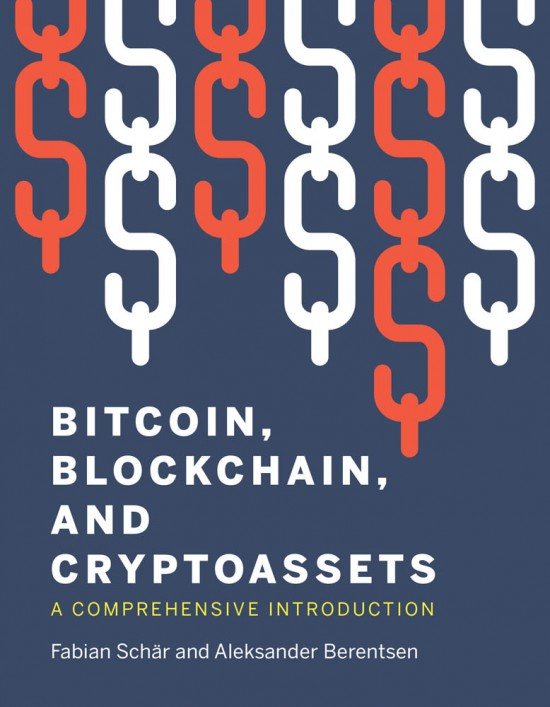
\includegraphics[width = 1.7cm, frame]{../assets/images/schaer_berentsen_cover}
			\end{column} %\hfill
			\begin{column}{0.8\textwidth}
				\textbf{Bitcoin, Blockchain and Cryptoassets} \\ 
				Fabian Schär and Aleksander Berentsen \\
				\texttt{ISBN: 978-0262539166}
			\end{column}
		\end{columns}
	}
	%
	\vspace{1.5em}
	%
	\uncover<2->{
		\begin{columns}[T]
			\begin{column}{0.1\textwidth}
					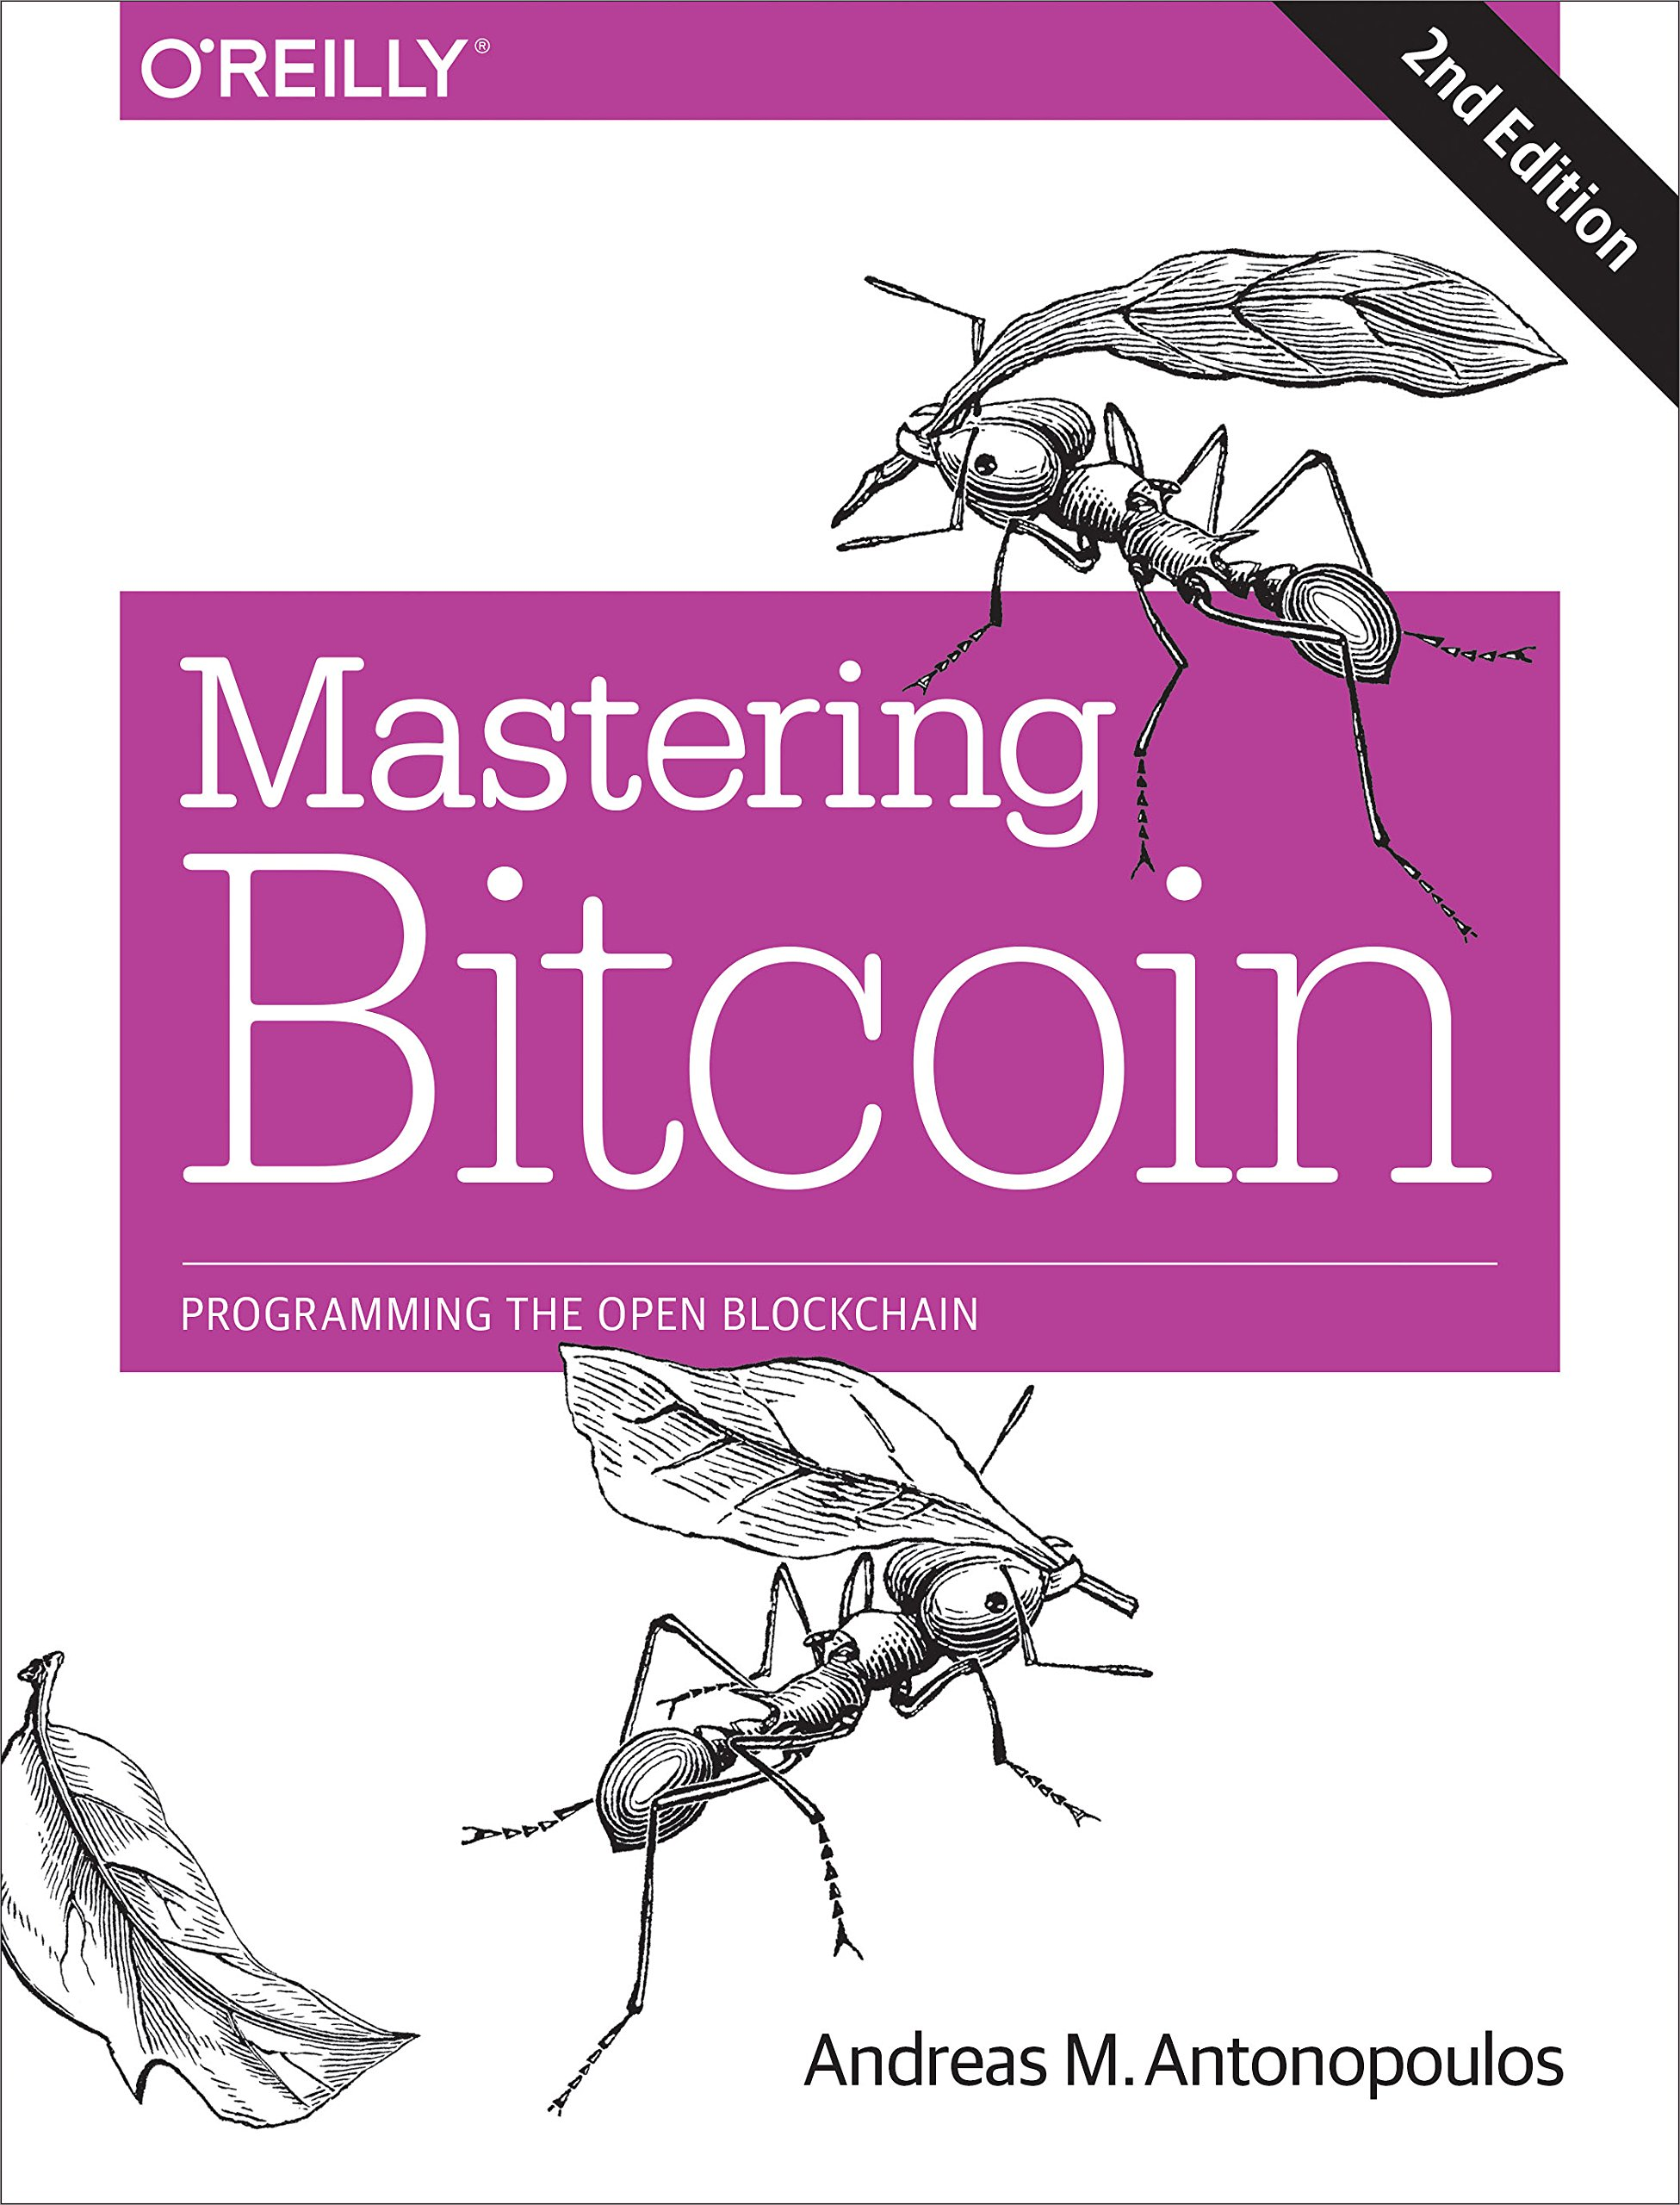
\includegraphics[width = 1.7cm, frame]{../assets/images/antonopoulos_cover}
			\end{column} %\hfill
			\begin{column}{0.8\textwidth}
				\textbf{Mastering Bitcoin - Second Edition}\\
				Andreas Antonopoulos\\
				\texttt{ISBN: 978-1491954386}
			\end{column}
		\end{columns}
	}
	%
	\vspace{1.5em}
	%
	\uncover<3->{
		\begin{columns}[T]
			\begin{column}{0.1\textwidth}
					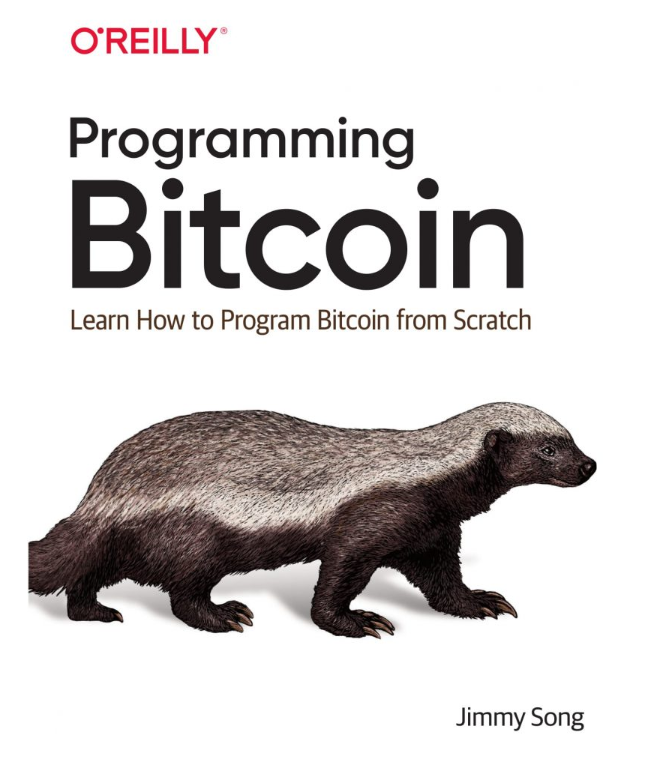
\includegraphics[width = 1.7cm, frame]{../assets/images/song_cover}
			\end{column} %\hfill
			\begin{column}{0.8\textwidth}
				\textbf{Programming Bitcoin}\\
				Jimmy Song\\
				\texttt{ISBN: 978-1492031499}
			\end{column}
		\end{columns}
	}
\end{frame}
%%%

%%%
\begin{frame}{Part of Multi-Course Series}

Blockchain courses have been part of the University of Basel's curriculum since 2017.

\vspace{1.5em}

\begin{columns}
	\begin{column}{0.35 \textwidth}
		\uncover<1->{
			\includegraphics[width = 4cm]{../config/logo_cif}
		}
	\end{column}
	\begin{column}{0.6 \textwidth}	
			\begin{itemize}
			\item<2-> This is a University undergrad-/ bachelor-level course
			\item<3-> It is part of a series of courses
			\item<4->  First course to switch to open lecture format
		\end{itemize}
	\end{column}	
\end{columns}

\vspace{2em}

\uncover<5->{
	$\rightarrow$ There is another open lecture course ``Smart Contracts and Decentralized Finance'' at the graduate-/master-level (\link \href{https://cryptolectures.teachable.com/p/smart-contracts-and-decentralized-finance}{link to course})
}

\end{frame}
%%%

%%%
\begin{frame}{Three Options to Take This Course}

The goal of our open lectures is to make teaching resources freely available. There are \color{focus} \textbf{three options} \color{black} for taking this course:\vspace{1em}

\begin{table}\footnotesize
	\begin{tabular}{lcccc}
	\hline \hline
									& Videos 		& Platform 		& Quizzes \& Exercise Sets 	& ECTS 	\\ \cline{2-5}
		YouTube 	 				& $\checkmark$	& 				& 				& 		\\
		Cryptolectures.io 			& $\checkmark$	& $\checkmark$	& $\checkmark$	&		\\
		University of Basel			& $\checkmark$	& $\checkmark$	& $\checkmark$	& $\checkmark$	\\
		\hline \hline
	\end{tabular}
\end{table} \vspace{2em}

\uncover<2->{
\link \href{https://www.youtube.com/watch?v=7oi06mvRB7M&list=PLoVRRjQbqYFw4wJ-oh-_iGPBiSvwDtUw0&index=2}
  {YouTube Channel}  \\
\link \href{http://www.cryptolectures.io}{Cryptolectures.io} \\
\link \href{https://www.unibas.ch/en/Studies/Application-Admission.html}{University of Basel - General Information}
}

\end{frame}
%%%

%%%
\begin{frame}{Quizzes and Exercise Sets}

	End-of-lecture quizzes and two exercise sets are available on the cryptolectures platform. Please note that these assessments are \textbf{not} graded and \textbf{entirely voluntary} for self-evaluation.

	\vspace{1em}
	
	\uncover<1->{
		\textbf{Quizzes:}
			\begin{itemize}
				\item Simple MC questions to test yourself
				\item At the end of each lecture on the cryptolectures platform
				\item \textbf{Not} graded
			\end{itemize}
	}
	
	\vspace{1em}
	
	\uncover<2->{
		\textbf{Exercise Sets:}
			\begin{itemize}
				\item PDFs on the cryptolectures platform
				\item Test yourself; the solutions are also available on cryptlectures.io
				\item \textbf{Not} graded
			\end{itemize}
	}
\end{frame}
%%%

%%%
\begin{frame}{Information for University of Basel Students}

	To earn 3 ECTS, you must pass the end-of-semester exam. Additionally, there is one voluntary mid-semester assignment that allows you to earn bonus points for the final exam.
	
	\vspace{1em}
	
	\uncover<1->{
	\textbf{Mid-Semester Assignment:}
	\begin{itemize}
		\item Similar to the exercise sets
		\item Will be published mid-semester on ADAM
		\item Bonus points for the exam if you hand-in correct solutions before deadline
	\end{itemize}
	
	\uncover<2->{
		\textbf{Exam:}
			\begin{itemize}
				\item 90 Minutes
				\item Closed book
				\item T/F, MC, Numbers and Text/Figure Boxes
				\item You may use a non-programmable calculator in accordance with the \link \href{https://wwz.unibas.ch/en/studies/examinations/use-of-materials-and-aids/}{faculty rules}.
				\item Any calculator that is not included on the faculty-approved list must not be used!
	\end{itemize}
	}	
	
}	
	
\end{frame}
%%%

%%%
\begin{frame}{Meet the Open Lectures Team}
	\begin{columns}[T]
		\begin{column}{0.31\textwidth}
			\center \textbf{Professor}
			\begin{table}\small
				\begin{tabular}{c}
					Fabian Schär\\
					\href{https://linkedin.com/in/fabian-schaer/}{\faLinkedinSquare}\ \href{https://twitter.com/fschaer}{\faTwitterSquare}\\
				\end{tabular}
			\end{table}
		\end{column}
		\begin{column}{0.31\textwidth}
			\center \textbf{PhD Candidate}
			\begin{table}\small
				\begin{tabular}{c}
					Dario Thürkauf\\
					\href{https://linkedin.com/in/dario-thuerkauf/}{\faLinkedinSquare} \href{https://twitter.com/dario_thuerkauf}{\faTwitterSquare}\\
				\end{tabular}
			\end{table}
		\end{column}
		\begin{column}{0.31\textwidth}
			\center \textbf{Student Assistants}
			\begin{table}\small
				\begin{tabular}{c}
					Andreas Arnold\\
					\href{https://www.linkedin.com/in/andreas-arnold-170a20225/}{\faLinkedinSquare}\ \href{}{\faTwitterSquare}\\
					\vspace{0.5em}\\
					Jonas Ruchti\\
					\href{https://www.linkedin.com/in/jonas-ruchti-a29042221/}{\faLinkedinSquare}\ \href{https://twitter.com/jonas_ruchti}{\faTwitterSquare}\\
				\end{tabular}
			\end{table}
		\end{column}
	\end{columns}
\end{frame}
%%%

\end{document}